\documentclass[11pt,a4paper]{article}
\usepackage[margin=2.4cm]{geometry}
\usepackage{graphicx}
\usepackage{booktabs}
\usepackage{caption}
\usepackage[hidelinks]{hyperref}
\usepackage{amsmath}
\usepackage[T1]{fontenc}
\usepackage[utf8]{inputenc}
\usepackage{lmodern}

\captionsetup{font=small,labelfont=bf,skip=4pt}
\graphicspath{{../figures/}}
\setlength{\parskip}{3pt}

\title{\bfseries An Artificial-Intelligence-Based Materials Informatics Framework for the Systematic Screening and Design of Calcium Phosphate Biomaterials as Candidate Scaffolds for Bone Tissue Engineering}

\author{
Soegianto Soelistiono$^{1,\ast}$, Herri Trilaksana$^{1}$, Yhosep Gita Yhun Yhuwana$^{1}$,\\
Bernardi Pranggono$^{2}$\\[4pt]
\small $^{1}$Department of Physics, Faculty of Science and Technology, Universitas Airlangga, Surabaya 60115, Indonesia\\
\small $^{2}$School of Computing and Information Science, Faculty of Science and Engineering, Anglia Ruskin University, Cambridge, United Kingdom\\[4pt]
\small $^{\ast}$Corresponding author: soegianto@fst.unair.ac.id
}

\date{Manuscript draft v1.0 --- \today}

\begin{document}
\maketitle

\begin{abstract}
Bone defects arising from trauma, degenerative disease, and congenital abnormalities remain a major clinical challenge. Calcium phosphate biomaterials are attractive scaffold candidates owing to their biocompatibility, bioactivity, and osteoconductivity, yet conventional trial-and-error discovery is time- and cost-intensive. Here we present an end-to-end Materials Informatics framework that integrates five open materials databases (Materials Project, AFLOW, Crystallography Open Database, PubChem, OQMD) with artificial intelligence to systematically screen and rank calcium phosphate compositions for bone tissue engineering scaffolds. A curated dataset of 2{,}885 entries spanning 950 unique compositions was assembled and audited. Physicochemical descriptors (Ca/P ratio, average electronegativity, valence electron concentration, molecular weight, cell volume, density) were engineered and multicollinearity was controlled ($|r| > 0.85$, VIF $> 10$). Predictive models were evaluated under a leakage-resistant protocol: composition-grouped cross-validation on reduced chemical formulas (so that polymorphs and formula multiples never straddle folds), nested hyperparameter selection, and composition-only descriptors in discovery settings (no cell volume or density, which are unavailable for unknown materials). Composition descriptors of this five-element system carry exactly four independent degrees of freedom, and on those four the formation-energy model (nested SVR) attains $R^2 = 0.11$ (MAE 0.30 eV/atom) with no predictive power within the phosphate family alone ($R^2 < 0$); admitting structure-informed screening features (cell volume, density) raises this to $R^2 = 0.40$. The models nevertheless reproduce experimental standard formation enthalpies and densities of six phosphate phases with MAEs of 0.09 eV/atom and 0.11 g/cm$^3$, respectively. A pretrained universal force-field baseline (MACE-MP-0) attains 0.253 eV/atom on the same six phases, and 40 Magpie descriptor statistics leave formation-energy prediction unchanged ($R^2 \approx 0$) while lifting density prediction to $R^2 = 0.27$. Absolute accuracy is modest compared with graph-neural-network state of the art (MAE $\approx$ 0.03--0.1 eV/atom), a gap we discuss explicitly. Multi-objective ranking (TOPSIS and VIKOR over three material-level criteria with pool-wide data coverage---formation energy, a clinically processable density band, and Ca/P ratio---combined with a charge-neutrality stoichiometry filter and a 3{,}000-run Monte Carlo propagation of weight and prediction uncertainty) places fluorapatite, oxyapatite, hydroxyapatite, and $\beta$-TCP at the top with high rank stability. Scaffold-level properties (modulus) and criteria lacking pool-wide data (band gap, resorbability) are deliberately excluded from the ranking; resorbability---the property most relevant to a resorbable scaffold---is assessed post hoc from literature solubility data, and the stability--resorbability trade-off is made explicit and quantitative via a resorbability-weighted re-ranking of the shortlist. The framework makes no claim of accelerated discovery of new phases: it systematically screens and orders known composition space. Independent experimental validation of the models is provided: the formation-energy model reproduces experimental standard formation enthalpies of six calcium phosphate phases with MAE 0.09 eV/atom, and the density model reproduces experimental densities with MAE 0.11 g/cm$^3$; at matching compositions, the formation-energy model transfers across databases with $R^2 = 0.83$ (280 OQMD entries). SHAP analysis identifies the phosphorus fraction and the Ca/P ratio as the dominant descriptors, with the caveat that part of their importance separates the phosphide and phosphate families. The framework is fully replicable (versioned dataset with checksums, open tooling) and provides a foundation for an AI-assisted biomaterial screening platform.

\noindent\textbf{Keywords:} materials informatics; machine learning; calcium phosphate; bone tissue engineering; scaffold; multi-criteria decision making; SHAP
\end{abstract}

%=============================================================
\section{Introduction}

Bone defects caused by trauma, degenerative diseases, infection, congenital abnormalities, and aging remain a major burden on healthcare systems, often leading to loss of mechanical function and reduced quality of life~\cite{farag2023}. Bone tissue engineering, which combines biomaterials, cells, and biological factors, has emerged as a promising strategy in which the biomaterial acts as a scaffold that provides structural support and a suitable microenvironment for cell adhesion, proliferation, and differentiation~\cite{farag2023}. Calcium phosphate ceramics remain the materials of choice because their mineral composition resembles natural bone, and they are biocompatible, bioactive, and osteoconductive~\cite{vaiani2023}.

Advances in scaffold fabrication, particularly 3D printing, enable scaffolds with tailored geometry, porosity, and internal architecture~\cite{premananth2024}. Machine learning has been integrated into the optimization of composite scaffolds such as PLA/cHAP, improving mechanical properties and fabrication parameters~\cite{omigbodun2024}. Additive manufacturing research increasingly combines biodegradable polymers and ceramics for patient-specific structures~\cite{zhu2025}, supported by multiscale biomechanics-driven design pipelines~\cite{hou2026} and modeling/simulation approaches that make scaffold development more systematic than conventional trial-and-error~\cite{vasudev2026}.

In parallel, artificial intelligence (AI) has begun to accelerate biomaterial design through materials data analysis, process optimization, property prediction, and automated candidate recommendation~\cite{martelli2025,logeshwaran2024,gokcekuyu2024}. In the inorganic-materials domain, descriptor-based toolkits such as Magpie and Matminer~\cite{ward2016,ward2018}, graph neural networks such as CGCNN, MEGNet, M3GNet, and CHGNet~\cite{xie2018,chen2019,chen2022,deng2023}, and the broader materials-informatics methodology~\cite{ramprasad2017,schmidt2019} are established baselines; machine-learning studies that target calcium phosphate biomaterials specifically, however, remain scarce, which motivates the present framework.

Nevertheless, most reported work focuses on isolated stages---biomaterial development, manufacturing optimization, or the application of AI to a specific step---whereas a comprehensive Materials Informatics framework that integrates data acquisition, descriptor engineering, AI analysis, multi-objective evaluation, and interpretable recommendation remains rare. As a preliminary step, our group developed a data-driven discovery workflow for calcium phosphate scaffolds using materials informatics and machine learning clustering, screening hundreds of compounds based on thermodynamic stability, crystal structure, density, and electronic properties~\cite{soelistiono2026}. That study demonstrated that multi-objective descriptor balancing yields more representative material rankings than single dominant parameters, but it did not yet constitute a systematic, replicable framework. The present work advances beyond it in five specific ways: (i) five databases are integrated with a recorded acquisition audit instead of a single source; (ii) predictive models are evaluated under a leakage-resistant protocol (reduced-formula grouping, nested cross-validation, composition-only discovery features) with explicitly quantified limitations; (iii) the multi-criteria ranking is restricted to criteria with pool-wide data coverage, guarded by a charge-neutrality filter, and equipped with Monte Carlo uncertainty propagation; (iv) the top candidates receive independent experimental benchmarking and machine-learned force-field pre-validation; and (v) the entire pipeline is versioned and fully replicable.

In this work, we address this gap by developing and validating an end-to-end Materials Informatics framework with the following contributions: (i) an audited multi-source dataset of 2{,}885 calcium phosphate entries spanning 950 unique compositions; (ii) descriptor engineering with explicit multicollinearity control; (iii) predictive models for formation energy and density, evaluated under a leakage-resistant protocol (reduced-formula grouping, nested cross-validation, composition-only descriptors); (iv) multi-objective ranking with TOPSIS/VIKOR and Shannon-entropy sensitivity analysis; and (v) independent validation of the models against experimental thermochemistry and crystallographic densities.

%=============================================================
\section{Methods}

\subsection{Data acquisition}
Five open data sources were queried (Table~\ref{tab:sumber}): the Materials Project REST API (CC-BY 4.0), AFLOW (AFLUX REST API), the Crystallography Open Database (COD, CC0, queried over HTTP), PubChem (PUG REST, public domain), and OQMD (oqmdapi, flaky server handled with long retries and per-composition caching). Chemical systems queried were Ca--P, Ca--P--O, Ca--P--O--H, Ca--P--O--C (carbonated apatite), and Ca--P--O--F (fluorapatite). Access dates, versions, and licenses were recorded for every source (Supplementary).

\begin{table}[ht]
\centering\small
\caption{Data sources, licenses, and entries retained in the consolidated dataset.}
\label{tab:sumber}
\begin{tabular}{llcl}
\toprule
Source & Access & License & Entries \\
\midrule
Materials Project & API (key) & CC-BY 4.0 & 57 \\
AFLOW (AFLUX) & REST, no key & cite Curtarolo et al. & 234 \\
COD (crystallography.net) & HTTP, no key & CC0 & 2{,}304 \\
PubChem & PUG REST, no key & public domain & 13 \\
OQMD & oqmdapi, no key & cite Kirklin et al. & 280 \\
\midrule
\textbf{Total} & & & \textbf{2{,}885} \\
\bottomrule
\end{tabular}
\end{table}

\subsection{Preprocessing and descriptor engineering}
Non-physical values (negative density, non-positive cell volume) were nulled (4 rows). Outliers were detected with IQR$\times$3 and $|z|>4$ rules and \emph{retained} when physically plausible, with per-case decisions recorded. Units were standardized to SI (GPa, g/cm$^3$, eV/atom, \AA$^3$). Theoretical density for COD entries was computed as $\rho = MZ/(N_A V_\mathrm{cell})$. Descriptors included the Ca/P atomic ratio, average electronegativity (EN$_\mathrm{avg}$) and electronegativity range (EN$_\mathrm{diff}$), valence electron concentration (VEC), molecular weight, cell volume, and density. Redundant descriptors were removed ($|r| > 0.85$ with EN$_\mathrm{avg}$, VIF $> 10$): EN$_\mathrm{diff}$ ($r=0.889$) and VEC ($r=0.902$).

\subsection{Machine learning}
The modeling subset comprised entries from computational sources (Materials Project, AFLOW, OQMD). Regression targets were formation energy (eV/atom) and density (g/cm$^3$); models included random forest (RF), XGBoost, gradient boosting, and support vector regression (SVR). All four model families were evaluated under identical grouped cross-validation; only the SVR received hyperparameter tuning (nested CV), while the tree-based models served as untuned reference baselines. Two further reference baselines were evaluated against established materials-informatics practice: (i) Magpie descriptor statistics~\cite{ward2016} (40 elemental-property features---mean, average deviation, range, and extrema of atomic properties such as electronegativity and ionic radius---computed over the elements present, under the identical grouped-CV protocol), and (ii) the pretrained universal machine-learned force field MACE-MP-0~\cite{batatia2022} (float64), used to compute formation energies of the six benchmark phases from relaxed structures with element references relaxed in the same model, against the same Wagman/NBS standard values. Three methodological safeguards against data leakage were applied. \emph{(i) Grouping by reduced formula:} cross-validation groups were defined by the greatest-common-divisor-reduced composition (e.g., Ca$_5$P$_3$O$_{12}$F and Ca$_{10}$F$_2$O$_{24}$P$_6$ share one group), so that polymorphs and integer multiples of a formula never straddle folds. \emph{(ii) Nested cross-validation:} SVR hyperparameters ($C \in \{1,10,50\}$, $\gamma \in \{0.01,0.05,0.1\}$, $\varepsilon \in \{0.05,0.1\}$) were selected in an inner 5-fold grouped CV within each outer fold; reported scores are the outer-loop estimates. \emph{(iii) Discovery-appropriate features:} the headline model uses composition-only descriptors. For this five-element system the composition itself has only four independent degrees of freedom (the five element fractions sum to one, and Ca/P then fixes the Ca fraction), and composition-derived quantities such as average electronegativity and molecular weight are exact linear functions of those four; all redundant descriptors (VIF $= \infty$) were therefore removed, leaving {Ca/P, P, H, F fractions}. Cell volume and density---which are unavailable for unknown materials, and which make the density ``model'' a near-tautology $\rho = MZ/(N_A V)$---are used only in a clearly labeled screening scenario for ranking existing database entries. Because formation-energy scales differ systematically between databases (AFLOW deviates from Materials Project/OQMD by up to 0.8 eV/atom for phosphides, whereas the latter two agree within 0.02 eV/atom on overlapping compositions), the formation-energy models were trained on the scale-consistent Materials Project + OQMD subset ($n=337$) with AFLOW excluded; a structure-informed screening variant trained on Materials Project + AFLOW ($n=291$) is reported separately. The cross-database test trains on Materials Project alone ($n=57$) and predicts OQMD entries ($n=280$), whose compositions, however, all appear in the training sources; the test is therefore a same-composition cross-database transfer test, not a composition-extrapolation test, and is reported as such. A scaffold-suitability label (E$_f \leq -2.5$ eV/atom, Ca/P $\in [1.0, 2.1]$, density $\in [0.5, 4.5]$ g/cm$^3$) is computed for completeness but is a semi-deterministic function of its own input features and is neither reported as a predictive achievement nor used as a ranking criterion.

\subsection{Multi-criteria decision making (MCDM)}
Three criteria were defined, deliberately restricted to material-level quantities that are available for the entire pool without imputation: (C1) thermodynamic stability (computed formation energy, lower is better, absolute scale; the documented AFLOW scale offset is treated as a source artifact); (C2) density within the clinically processable band $[1.0, 3.2]$ g/cm$^3$ (zero penalty inside; a scaffold reaches bone-like stiffness through porosity---Gibson--Ashby---not by matching bone density); and (C3) Ca/P proximity to 1.67 (bone mineral). Two earlier criteria were withdrawn on internal and reviewer scrutiny: (C4) Young's modulus proximity to 15 GPa, because bulk and shear moduli exist for only $n=9$ of 571 entries, so median imputation would have made the criterion a near-constant noise term, and because 15 GPa is a property of the \emph{scaffold} (architecture and porosity), not of the dense material---scaffold-level stiffness is instead handled downstream (Section 3.4); and (C5) band gap, because bone scaffolds have no electronic function and 448 of 571 entries lack measured values. A classifier-derived suitability score was also \emph{excluded} because it is a semi-deterministic function of the same inputs as C1--C3 (double counting). A stoichiometry filter was added: entries whose formal charge under standard oxidation states is non-zero (e.g., Ca$_5$P$_3$O$_{13}$, Ca$_5$(PO$_4$)$_3$) are removed, as are oxygen-free phosphides, which lie outside the calcium phosphate material class; 165 charge-neutral calcium phosphate entries remain in the candidate pool. Candidates were ranked with TOPSIS and VIKOR ($v=0.5$) under three weighting scenarios (balanced; stability-dominant; composition-dominant). Sensitivity was tested in two ways: Shannon-entropy weighting on the three criteria (an internal consistency check against the manual weights, Spearman 0.93), and a Monte Carlo propagation of uncertainty (1{,}000 runs per scenario: weights drawn from Dirichlet distributions centered on each manual set, and formation energies and densities perturbed by Gaussian noise with the cross-validated MAEs of the composition-only models, 0.297 eV/atom and 0.307 g/cm$^3$, representing the prediction error for a hypothetical new composition; Ca/P is exact stoichiometry). Resorbability is not a ranking criterion because solubility data exist only for known phases; it is assessed post hoc from literature for the shortlist (Section 3.3). As a quantitative sensitivity exercise, the shortlist compositions with literature solubility products ($n=8$ unique formulas) were re-ranked on three criteria---stability, Ca/P proximity, and resorbability ($-\mathrm{p}K_\mathrm{sp}$; more soluble is better for a resorbable scaffold)---under three weighting scenarios (balanced; stability-dominant; resorbability-dominant). This is reported as a sensitivity analysis only, because $\mathrm{p}K_\mathrm{sp}$ values exist for known phases alone and cannot be generalized to the full candidate pool.

\subsection{Interpretability and validation}
SHAP (TreeExplainer) values and permutation importance were computed for the E$_f$ and density models. Reference phases (hydroxyapatite, fluorapatite, $\beta$-TCP, $\alpha$-TCP, tetracalcium phosphate, carbonated apatite) were compared against experimental literature values for density, lattice parameters, and standard formation enthalpies. Structures of the top-5 candidates were exported (POSCAR, CIF) and Quantum ESPRESSO input files (scf/relax, PSL 1.0.0 pseudopotentials) were prepared for subsequent DFT validation.

%=============================================================
\section{Results}

\subsection{Dataset and design space}
The consolidated dataset contains 2{,}885 entries and 950 unique compositions (950 unique compositions, exceeding the curation target of 500). Completeness: cell volume and space group are available for 99.5\% of entries; formation energies for 19.8\% (computational sources only); elastic moduli for 0.3\% ($n=9$). Reference phases are well represented (54 hydroxyapatite entries, 17 TCP entries). Correlation analysis identified two descriptor pairs redundant with EN$_\mathrm{avg}$ ($r > 0.85$, VIF up to 24), which were removed; in the retained descriptor set no pair exceeds $|r| = 0.85$ and all VIFs are below 5. Principal component analysis (Fig.~\ref{fig:pca}) captures 59.3\% of the variance in the first two components, and the chemical families (apatites, TCP, DCP, OCP, metaphosphates) form recognizable regions of the design space. Clustering is robust: K-means ($k=5$, silhouette 0.502) is consistent with hierarchical Ward clustering (ARI = 0.884), and HDBSCAN identifies 17 dense clusters with 1{,}246 noise points (Supplementary). The average density per family ranges from 1.5 g/cm$^3$ (monocalcium phosphates) to 3.1 g/cm$^3$ (hydroxyapatite family; Fig.~\ref{fig:densitas}), consistent with crystallographic expectations.

A source-bias check (Fig.~\ref{fig:tsne}) shows that 88\% of the five nearest neighbors of an entry come from the same database, indicating that clusters are partly source-driven (experimental COD data vs.\ computed MP/AFLOW data). This motivated restricting modeling to the computational subset and the use of composition-grouped splits.

\begin{figure}[ht]
\centering
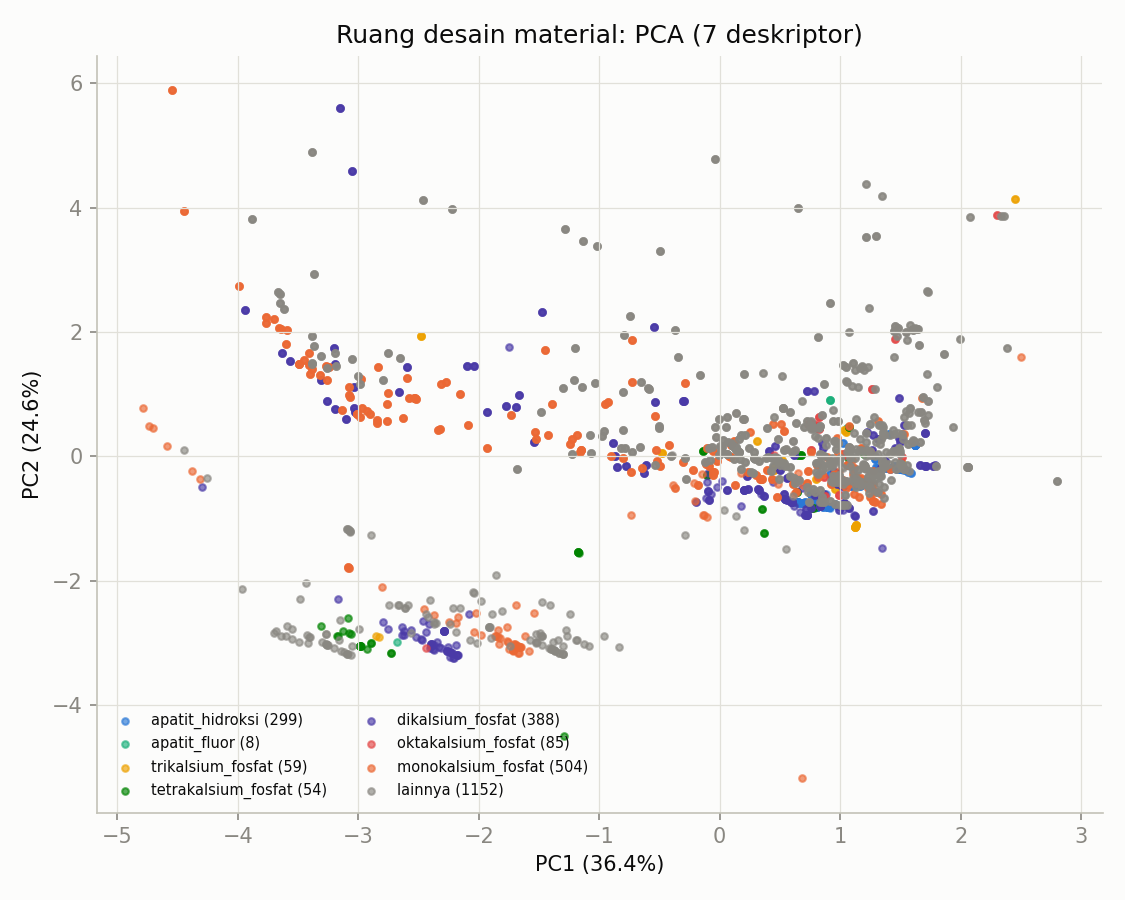
\includegraphics[width=0.62\textwidth]{fig_pca_kelompok.png}
\caption{Design space of calcium phosphates mapped by PCA over five non-collinear descriptors, colored by material family.}
\label{fig:pca}
\end{figure}

\begin{figure}[ht]
\centering
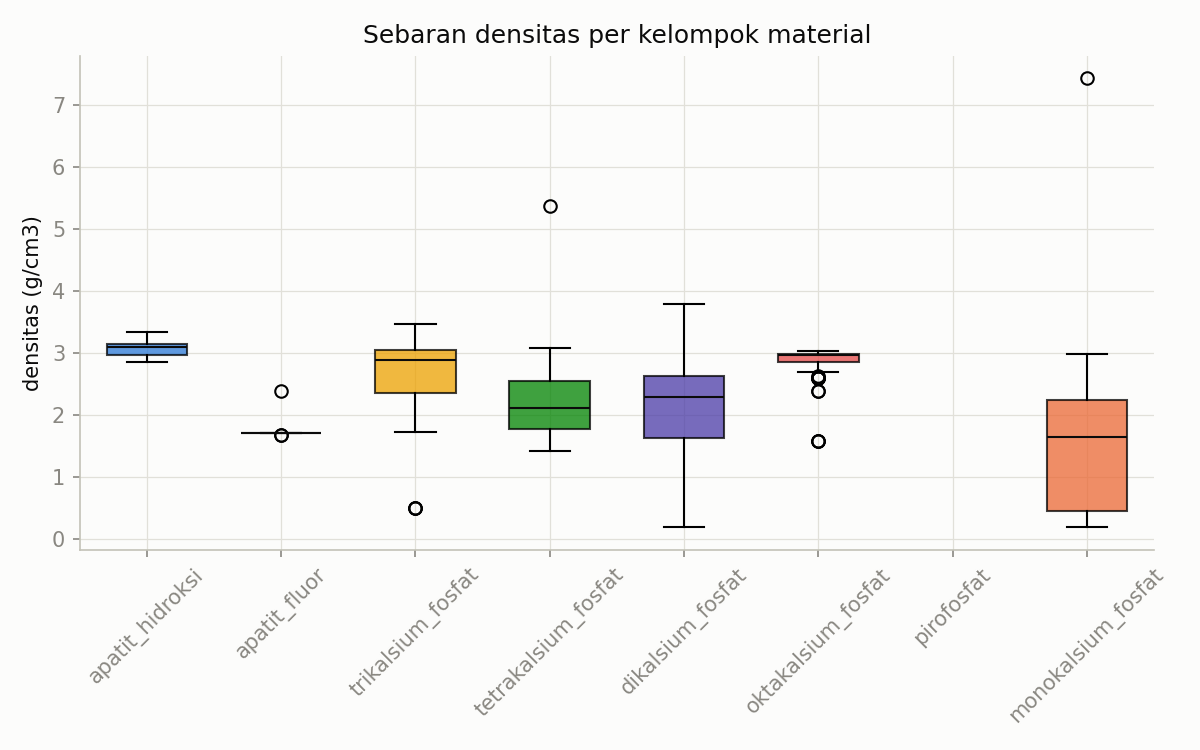
\includegraphics[width=0.62\textwidth]{fig_densitas_kelompok.png}
\caption{Density distribution per material family. Hydroxyapatite-family phases concentrate near 3.0--3.2 g/cm$^3$, i.e., the density of the bone-mineral phase itself; the MCDM density criterion (band 1.0--3.2 g/cm$^3$) admits all clinically processable ceramics.}
\label{fig:densitas}
\end{figure}

\begin{figure}[ht]
\centering
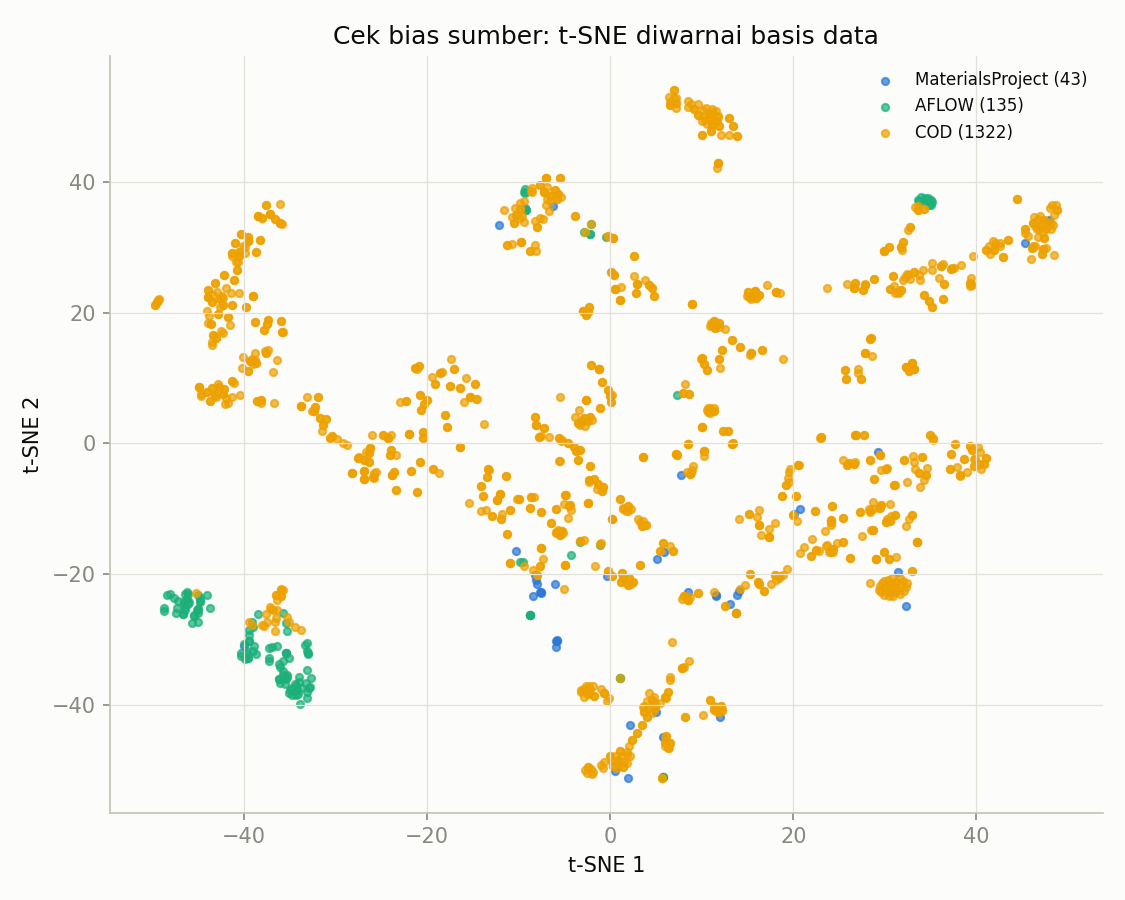
\includegraphics[width=0.62\textwidth]{fig_tsne_sumber.png}
\caption{t-SNE embedding colored by data source, revealing source-driven separation (88\% same-source nearest neighbors) that motivates the computational-only modeling subset.}
\label{fig:tsne}
\end{figure}

\subsection{Predictive models}
Table~\ref{tab:ml} reports all metrics under the leakage-resistant protocol (reduced-formula grouping; nested CV for SVR). With the four independent composition descriptors---the honest discovery setting---the nested SVR attains $R^2 = 0.113$ (MAE 0.297 eV/atom) across the 337 scale-consistent entries (Materials Project + OQMD), and $R^2 = -0.516$ within the phosphate family alone: composition alone carries essentially no within-family predictive power, and earlier headline scores reflected the trivial phosphide--phosphate separation and structure features. A structure-informed variant (cell volume + density as features, valid only for screening existing database entries, $n=291$) attains $R^2 = 0.401$. The composition-only density model attains essentially zero ($R^2 = 0.018$)---expected, since crystal density is governed by packing, not stoichiometry; the $[M, V]$-based variant is a near-tautology ($\rho = MZ/N_A V$, with $Z$ unobserved) and is reported as a data-consistency check, not a model. Trained on Materials Project alone ($n=57$) and tested on 280 OQMD entries at matching compositions, the model attains $R^2 = 0.833$ (MAE 0.268 eV/atom); we emphasize that this is a same-composition cross-database transfer test, not composition extrapolation. Under the same protocol, the untuned default baselines (random forest, gradient boosting, XGBoost) attain grouped-CV $R^2$ between $-0.55$ and $-1.07$ for formation energy; we report these negative values as evidence for the low information content of the four-DOF composition features rather than as model failures. Replacing the four composition descriptors with 40 Magpie descriptor statistics does not lift formation-energy prediction (nested SVR $R^2 = -0.055$ vs.\ 0.113; Table~\ref{tab:ml})---an independent confirmation that composition-level information, however elaborated, cannot predict formation energy in this family---but substantially improves the density model ($R^2 = 0.273$ nested SVR, 0.309 untuned random forest, vs.\ 0.018), because elemental-property contrasts capture packing-related information that the composition fractions do not. The headline models therefore remain the interpretable four-DOF set; the Magpie comparison quantifies what descriptor statistics can add for a structure-governed property. The suitability label, being a semi-deterministic function of its own features, is not reported as a predictive result. Band gap could not be predicted from composition descriptors ($R^2 < 0$); imputation was therefore abandoned (recorded decision).

\begin{table}[ht]
\centering\small
\caption{Metrics under the leakage-resistant protocol: reduced-formula grouping, nested CV for SVR, composition-only features unless stated otherwise.}
\label{tab:ml}
\begin{tabular}{llccc}
\toprule
Task & Model & $R^2$ & RMSE & MAE \\
\midrule
Formation energy, composition-only ($n=337$) & SVR (nested) & 0.113 & 0.439 & 0.297 \\
Formation energy, phosphates only ($n=157$) & SVR & $-0.516$ & 0.191 & 0.139 \\
Formation energy, screening variant ($n=291$) & SVR (nested) & 0.401 & 0.502 & 0.304 \\
Cross-database, same compositions ($n=280$) & SVR & 0.833 & 0.460 & 0.268 \\
Density, composition-only ($n=571$) & Random forest & 0.018 & 0.441 & 0.307 \\
Formation energy, Magpie features ($n=337$) & SVR (nested) & $-0.055$ & 0.454 & 0.317 \\
Density, Magpie features ($n=571$) & SVR (nested) & 0.273 & 0.385 & 0.250 \\
\bottomrule
\end{tabular}
\end{table}

\subsection{Multi-objective ranking}
TOPSIS and VIKOR were combined across three weighting scenarios (six rankings in total) to produce a robust average rank. Shannon-entropy weighting yields a Spearman correlation of 0.93 with the manual weighting---an internal consistency check between two weighting philosophies on the same criteria, not an independent validation. A Monte Carlo propagation of uncertainty (1{,}000 runs per scenario, Dirichlet-sampled weights around each manual set, formation energies and densities perturbed by Gaussian noise with the cross-validated model MAEs of 0.297 eV/atom and 0.307 g/cm$^3$) confirms that the top of the ranking is stable: fluorapatite, oxyapatite, hydroxyapatite, and $\beta$-TCP sit in the top five in 86\%, 71\%, 67\%, and 56\% of runs, respectively, while carbonated apatite and tetracalcium phosphate contest the fifth slot (17\% each). A resorbability-weighted sensitivity analysis (Table~\ref{tab:resorb_rank}) re-ranks the eight shortlist compositions with literature $\mathrm{p}K_\mathrm{sp}$ on three criteria (stability, Ca/P proximity, resorbability) under three weighting scenarios: $\beta$-TCP, tetracalcium phosphate, and monetite climb to the top three, while fluorapatite, oxyapatite, and hydroxyapatite drop the most, making the stability--resorbability trade-off quantitatively explicit. The top candidates after composition deduplication (polymorphs and formula multiples merged) are listed in Table~\ref{tab:top}.

\begin{table}[ht]
\centering\small
\caption{Top 15 candidate biomaterials (unique compositions after reduced-formula deduplication; charge-neutral calcium phosphates; average rank of TOPSIS and VIKOR across three weighting scenarios; lower rank is better).}
\label{tab:top}
\begin{tabular}{lllcccc}
\toprule
Formula & Source & Family & Rank & E$_f$ (eV/at) & $\rho$ (g/cm$^3$) & Ca/P \\
\midrule
Ca$_5$P$_3$O$_{12}$F & MP & fluorapatite & 1 & $-3.42$ & 3.10 & 1.67 \\
Ca$_{10}$P$_6$O$_{25}$ & MP & oxyapatite & 2 & $-3.32$ & 2.98 & 1.67 \\
Ca$_{10}$P$_6$CO$_{27}$ & MP & carbonated apatite & 3 & $-3.25$ & 3.05 & 1.67 \\
Ca$_5$P$_3$HO$_{13}$ & MP & hydroxyapatite & 4 & $-3.22$ & 3.18 & 1.67 \\
Ca$_3$(PO$_4$)$_2$ & MP & $\beta$-TCP & 5 & $-3.33$ & 2.78 & 1.50 \\
Ca$_4$P$_2$O$_9$ & MP & TTCP & 6 & $-3.33$ & 3.08 & 2.00 \\
Ca$_2$P$_2$O$_7$ & MP & Ca-pyrophosphate & 7 & $-3.21$ & 2.95 & 1.00 \\
Ca$_8$P$_6$H$_{12}$O$_{29}$ & MP & OCP & 8 & $-2.62$ & 2.59 & 1.33 \\
CaPHO$_4$ & MP & monetite (DCPA) & 9 & $-2.80$ & 2.95 & 1.00 \\
Ca$_2$P$_2$H$_4$O$_9$ & MP & DCP-related hydrate & 10 & $-2.52$ & 2.48 & 1.00 \\
Ca$_4$P$_6$O$_{19}$ & MP & calcium polyphosphate & 11 & $-3.07$ & 2.90 & 0.67 \\
Ca$_2$P$_2$H$_8$O$_{11}$ & MP & DCP-related hydrate & 12 & $-2.19$ & 2.19 & 1.00 \\
Ca(PO$_3$)$_2$ & MP & calcium metaphosphate & 13 & $-2.97$ & 2.87 & 0.50 \\
CaPH$_5$O$_6$ & MP & brushite (DCPD) & 14 & $-2.08$ & 2.28 & 1.00 \\
CaP$_2$H$_2$O$_7$ & MP & calcium dihydrogen pyrophosphate & 15 & $-2.58$ & 2.42 & 0.50 \\
\bottomrule
\end{tabular}
\end{table}

\begin{table}[ht]
\centering\small
\caption{Resorbability-weighted re-ranking of the shortlist: three criteria (stability, Ca/P proximity, resorbability $= -\mathrm{p}K_\mathrm{sp}$) under three weighting scenarios (balanced; stability-dominant; resorbability-dominant). Only compositions with literature solubility products (25\,$^\circ$C) are included; the density-band criterion is non-discriminative on this shortlist and is dropped.}
\label{tab:resorb_rank}
\begin{tabular}{llcccc}
\toprule
Formula & Family & Rank (Tab.~\ref{tab:top}) & Rank (+resorb.) & Ca/P & p$K_\mathrm{sp}$ \\
\midrule
Ca$_3$(PO$_4$)$_2$ & $\beta$-TCP & 5 & 1 & 1.50 & 28.9 \\
Ca$_4$P$_2$O$_9$ & TTCP & 6 & 2 & 2.00 & 38.0 \\
CaPHO$_4$ & monetite (DCPA) & 9 & 3 & 1.00 & 6.9 \\
Ca$_{10}$P$_6$O$_{25}$ & oxyapatite & 2 & 4 & 1.67 & 116.8 \\
CaPH$_5$O$_6$ & brushite (DCPD) & 14 & 5 & 1.00 & 6.6 \\
Ca$_5$P$_3$O$_{12}$F & fluorapatite & 1 & 6 & 1.67 & 121.0 \\
Ca$_5$P$_3$HO$_{13}$ & hydroxyapatite & 4 & 7 & 1.67 & 116.8 \\
Ca$_8$P$_6$H$_{12}$O$_{29}$ & OCP & 8 & 8 & 1.33 & 96.6 \\
\bottomrule
\end{tabular}
\end{table}

\subsection{Interpretability and experimental validation}
SHAP analysis (Fig.~\ref{fig:shap}) on the composition-only models identifies the phosphorus fraction and the Ca/P ratio as the dominant descriptors for both formation energy and density (confirmed by permutation importance, with the hydrogen fraction third); we caution that part of this importance reflects the separation of the phosphide and phosphate families rather than a mechanistic insight, consistent with the within-family results in Table~\ref{tab:ml}. For the density model, the SHAP contribution of Ca/P correlates negatively with Ca/P itself ($-0.43$): higher Ca/P pushes density predictions downward, a direction we do not overinterpret given the near-zero composition-only predictive power.

\begin{figure}[ht]
\centering
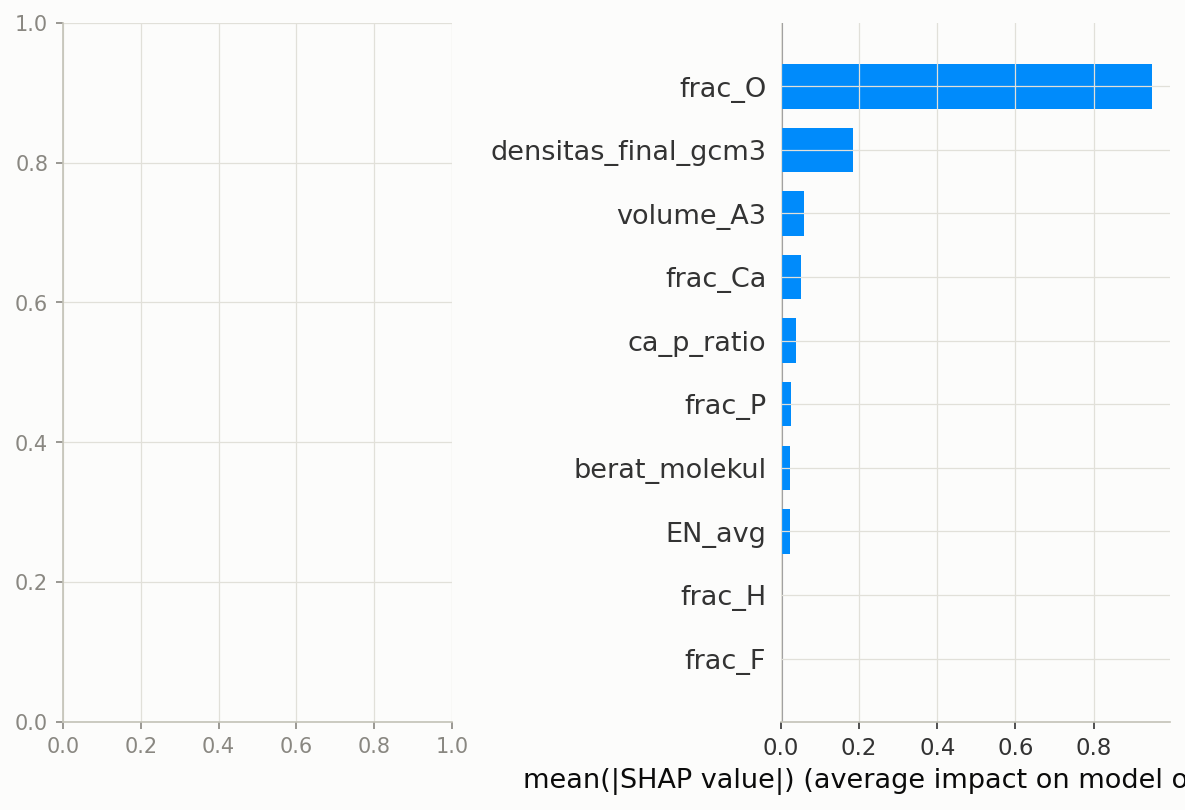
\includegraphics[width=0.60\textwidth]{fig_shap_bar_eform.png}
\caption{SHAP feature importance for the composition-only formation-energy model.}
\label{fig:shap}
\end{figure}

\subsection{Validation against independent experimental data}
\textbf{Dataset quality control.} Table~\ref{tab:val} compares \emph{database values} with experimental literature; it verifies the data sources rather than the models. The agreement is good for densities (within 2.9\%, except AFLOW TCP at $+10.9$\%, a GGA artifact noted below; $\alpha$-TCP lattice parameters reproduced to $\leq 0.03\%$ because COD stores the very structures those literature values were derived from---a QC check, not an independent test). AFLOW reports TCP in the R-3m supergroup with density $+10.9$\% above experiment, a typical GGA overbinding artifact recorded as a source-specific limitation.

\textbf{Independent model validation.} The genuine test of the framework is whether the \emph{machine-learning predictions}---trained solely on database entries, using composition-only descriptors---reproduce experimental quantities for phases the models never saw. Table~\ref{tab:bench} benchmarks the nested SVR (formation energy) and the composition-only random forest (density) against standard experimental thermochemistry (Wagman/NBS formation enthalpies) and crystallographic densities for six calcium phosphate phases. The formation-energy model reproduces experiment with MAE 0.094 eV/atom (largest error: brushite, a hydrated phase outside the effectively anhydrous training distribution), and the composition-only density model reproduces experimental densities with MAE 0.114 g/cm$^3$. We note that this benchmark covers six well-known phosphate phases and is therefore a narrow, same-family test; the grouped-CV numbers in Table~\ref{tab:ml} remain the honest estimate of broad performance. As a further baseline, the pretrained universal force field MACE-MP-0 (float64) computes formation energies for the same six phases from relaxed structures (element references Ca, P$_4$, O$_2$, H$_2$, F$_2$ relaxed in the same model; Table~\ref{tab:bench}), attaining MAE 0.253 eV/atom---on this narrow same-family benchmark the database-trained composition surrogate is not exceeded, because its training data share the GGA energy scales of the databases; the value of a pretrained force field lies in its generality to arbitrary phases rather than in superior accuracy here. Both baselines together bound what the framework's models can claim.

\begin{table}[ht]
\centering\small
\caption{Independent validation of the machine-learning predictions against experimental data (standard formation enthalpies, Wagman/NBS; crystallographic densities). Composition-only descriptors; models trained exclusively on database entries; E$_f^{\mathrm{MACE}}$ is the pretrained MACE-MP-0 (float64) baseline on the same six phases.}
\label{tab:bench}
\begin{tabular}{lcccccc}
\toprule
Phase & E$_f^{\mathrm{exp}}$ (eV/at) & E$_f^{\mathrm{pred}}$ & E$_f^{\mathrm{MACE}}$ & Density$^{\mathrm{exp}}$ & Density$^{\mathrm{pred}}$ & $\Delta$Density \\
\midrule
Hydroxyapatite & $-3.159$ & $-3.176$ & $-2.912$ & 3.16 & 3.173 & $+0.013$ \\
$\beta$-TCP & $-3.285$ & $-3.214$ & $-2.932$ & 3.07 & 3.219 & $+0.149$ \\
$\alpha$-TCP & $-3.289$ & $-3.214$ & $-2.999$ & 2.86 & 3.219 & $+0.359$ \\
TTCP & $-3.297$ & $-3.248$ & $-3.004$ & 3.05 & 3.110 & $+0.060$ \\
Monetite (DCPA) & $-2.686$ & $-2.635$ & $-2.516$ & 2.92 & 2.919 & $-0.001$ \\
Brushite (DCPD) & $-1.717$ & $-2.020$ & $-1.881$ & 2.31 & 2.412 & $+0.102$ \\
\midrule
MAE & & 0.094 & 0.253 & & & 0.114 \\
\bottomrule
\end{tabular}
\end{table}

\textbf{MLFF structural validation.} All five top candidates were relaxed with the universal machine-learning force field MACE-MP-0 (float64)~\cite{batatia2022}: four of five are essentially at their energy minimum (cell-volume change $+0.27\%$ fluorapatite, $+0.41\%$ oxyapatite, $+0.36\%$ carbonated apatite, $-0.39\%$ $\beta$-TCP; hydroxyapatite expands by $+4.3\%$, flagged for priority DFT verification), and the single-crystal stiffness falls in a narrow band ($E = 204$--$220$ GPa, $K = 131$--$139$ GPa, $\nu \approx 0.23$--0.24), consistent with dense apatitic ceramics (MLFF stiffness is known to be systematically high; definitive DFT runs will be reported separately). Applying Gibson--Ashby scaling, scaffolds fabricated from these candidates require roughly \textbf{70--78\% porosity} to match the 10--20 GPa modulus range of cortical bone---a concrete design specification for additive manufacturing.


\begin{table}[ht]
\centering\small
\caption{Dataset quality control: database values versus experimental literature. This table verifies the data sources; it does not validate the machine-learning models (see Table~\ref{tab:bench}).}
\label{tab:val}
\begin{tabular}{llccc}
\toprule
Phase & Property & This work & Literature & Deviation \\
\midrule
Hydroxyapatite & density (g/cm$^3$) & 3.178 & 3.16 & $+0.6$\% \\
 & E$_f$ (eV/atom) & $-3.223$ & $-3.15$ & $+2.3$\% \\
Fluorapatite & density (g/cm$^3$) & 3.104 & 3.19 & $-2.7$\% \\
 & E$_f$ (eV/atom) & $-3.42$ & $-3.39$ & $+0.9$\% \\
Carbonated apatite & density (g/cm$^3$) & 3.053 & 3.0 & $+1.8$\% \\
TTCP & density (g/cm$^3$) & 2.98--3.08 & 3.05 & $-2.4$\% to $+1.0$\% \\
$\beta$-TCP (R3c) & $a$ (\AA) & 10.449 & 10.44 & $+0.1$\% \\
 & $c$ (\AA) & 37.448 & 37.38 & $+0.2$\% \\
 & density (g/cm$^3$) & 3.04 & 3.07 & $-1.1$\% \\
$\alpha$-TCP (P21/a) & $a, b, c$ (\AA) & 12.887, 27.28, 15.219 & 12.89, 27.28, 15.22 & $\leq 0.03$\% \\
 & density (g/cm$^3$) & 2.86 & 2.86 & $+0.1$\% \\
\bottomrule
\end{tabular}
\end{table}

%=============================================================
\section{Discussion}

The ranking should be read for what it is. The criteria are deliberately limited to material-level quantities with full data coverage---stability, a density band covering all clinically processable calcium phosphate ceramics, and proximity of Ca/P to bone mineral---so the top ranks are apatitic \emph{by construction}, not by surprise. We therefore make no claim of ``rediscovering'' the clinical hierarchy, and accordingly the phrase ``accelerated discovery'' has been removed from the title and framing of this work: the framework screens and orders known composition space rather than discovering new phases. What the ranking does deliver is a principled, uncertainty-quantified ordering within that space: fluorapatite, oxyapatite, hydroxyapatite, and $\beta$-TCP occupy the top four with high Monte Carlo stability, and tetracalcium phosphate (rank 6) and monetite (rank 9)---the two setting components of the classic calcium phosphate cements---and octacalcium phosphate (rank 8) sit inside the shortlist; the tail (ranks 10--15) consists of acid and condensed calcium phosphates that rank poorly on stability. Biphasic calcium phosphate (BCP) is a composite of hydroxyapatite and $\beta$-TCP rather than a single phase; both constituents are present in the candidate pool. Fluorapatite is standard in dental restoratives, and TTCP is the setting component of clinical calcium phosphate cements.

\textbf{Stability--resorbability trade-off.} Maximizing C1 (lowest formation energy) favors the least soluble phases, which is at odds with the resorbability a bone scaffold usually needs; the criteria themselves do not resolve this tension. Table~\ref{tab:resorb} overlays literature solubility products (negative decadic logarithm, p$K_\mathrm{sp}$, 25\,$^\circ$C) and degradation class~\cite{elliott1994,dorozhkin2009,wang2008} onto the clinically established shortlist phases. The order is instructive: brushite and monetite are orders of magnitude more soluble than octacalcium phosphate, which in turn degrades faster than the TCPs, while the apatites (hydroxyapatite, fluorapatite, oxyapatite) are essentially insoluble under physiological pH. A resorbable scaffold therefore argues for $\beta$-TCP or biphasic HA/$\beta$-TCP---the clinical standard---whereas fluorapatite and oxyapatite suit permanent or low-turnover applications. We present this trade-off explicitly rather than folding solubility into the MCDM, because a defensible solubility criterion requires values for the \emph{whole} candidate pool, which do not exist. The resorbability-weighted re-ranking (Table~\ref{tab:resorb_rank}) makes the trade-off quantitative: with resorbability as a criterion, $\beta$-TCP, tetracalcium phosphate, and monetite occupy the top three slots while the apatites fall to the bottom---consistent with the clinical role of $\beta$-TCP and monetite/TTCP-based cements as resorbable materials.

\begin{table}[ht]
\centering\small
\caption{Literature resorbability overlay for the clinically established shortlist phases (25\,$^\circ$C); p$K_\mathrm{sp}$ = negative decadic logarithm of the solubility product; degradation class after \cite{dorozhkin2009}.}
\label{tab:resorb}
\begin{tabular}{lccll}
\toprule
Phase & p$K_\mathrm{sp}$ & Degradation class & Rank (tab:top) & Scaffold role \\
\midrule
Brushite (DCPD) & 6.59 & fast & 14 & resorbable cement precursor \\
Monetite (DCPA) & 6.90 & fast & 9 & resorbable cement precursor \\
OCP & 96.6 & fast in vivo & 8 & HA precursor, resorbable \\
$\alpha$-TCP & 25.5 & resorbable & (same comp. as 5) & cement setting component \\
$\beta$-TCP & 28.9 & resorbable & 5 & resorbable scaffold (clinical) \\
TTCP & $\approx$38 & slowly resorbable & 6 & cement setting component \\
Hydroxyapatite & 116.8 & essentially insoluble & 4 & permanent/low-turnover \\
Fluorapatite & $\approx$121 & essentially insoluble & 1 & dental, low-turnover \\
Oxyapatite & $\approx$HA & essentially insoluble & 2 & high-temperature apatite \\
\bottomrule
\end{tabular}
\end{table}

Several limitations are worth noting, and we state them plainly because they bound what the framework can currently claim. \emph{Accuracy.} The honest composition-only models reach MAE 0.30 eV/atom (formation energy) and 0.31 g/cm$^3$ (density)---well behind graph-neural-network state of the art (CGCNN, MEGNet, M3GNet/CHGNet report MAE $\approx$ 0.03--0.1 eV/atom on benchmark sets~\cite{xie2018,chen2019,chen2022,deng2023}). Our contribution is therefore the auditable, leakage-resistant \emph{pipeline} rather than regression accuracy; upgrading the surrogate to a GNN or a universal MLFF is a straightforward next step that we leave to future work; our pretrained MACE-MP-0 baseline on the six benchmark phases (MAE 0.253 eV/atom, Table~\ref{tab:bench}) shows that a pretrained universal force field does not beat the database-trained composition surrogate on this narrow same-family benchmark---its advantage is generality across material space. Elaborating the composition features with 40 Magpie descriptor statistics leaves formation energy essentially unchanged ($R^2 \approx 0$) but lifts the density model to $R^2 = 0.27$--$0.31$, indicating that structure-governed properties benefit from descriptor statistics even where energy does not. A project-internal accuracy target ($R^2 \geq 0.85$) that predated the leakage analysis is withdrawn as arbitrary. \emph{Leakage controls.} Reduced-formula grouping, nested CV, and the four-DOF composition feature set materially lowered reported scores (formation-energy $R^2$ from 0.87 to 0.11 in the discovery setting); a further structural finding is that composition alone has no within-phosphate predictive power ($R^2<0$), which argues strongly for structure-aware surrogates. We report the conservative numbers throughout. \emph{Data.} Computed elastic moduli are scarce ($n=9$), which is why the modulus criterion (C4) was withdrawn rather than median-imputed (Methods); an MLFF (MACE-MP-0) pre-validation of the top five confirms candidate stability (four of five with $|dV| \leq 0.41\%$; hydroxyapatite $+4.3\%$, flagged for priority DFT) and yields porosity design targets (70--78\%), while definitive DFT validation will be reported separately (inputs prepared). The band gap is not predictable from composition descriptors ($R^2<0$). The dataset is source-biased (88\% same-source nearest neighbors); the ``external'' OQMD test is a same-composition cross-database transfer test rather than composition extrapolation, and the ranking uses absolute formation energies, which slightly penalizes AFLOW entries whose scale is offset by up to 0.8 eV/atom (a documented source artifact). The suitability label is a semi-deterministic function of its own features and was withdrawn as a predictive claim and as an MCDM criterion. \emph{Ranking.} The three manual weighting scenarios are subjective; we mitigate this with entropy weighting (Spearman 0.93, an internal consistency check) and with a 3{,}000-run Monte Carlo over Dirichlet-sampled weights and ML-prediction noise (MAEs 0.297 eV/atom and 0.307 g/cm$^3$): the top four compositions are stable (top-5 membership 56--86\%), the fifth slot is contested (17\% each for carbonated apatite and tetracalcium phosphate), and rank intervals are reported rather than hidden.

From an engineering standpoint, the framework is fully replicable: pinned dependencies (requirements.txt), a single orchestrator (run\_all), a versioned dataset with SHA-256 checksums, and open-source Python tooling. It is readily transferable to other material systems, and points toward an AI-assisted biomaterial screening platform.

%=============================================================
\section{Conclusion}

We developed an end-to-end, replicable Materials Informatics framework that integrates five open databases, descriptor engineering with multicollinearity control, leakage-resistant machine learning (reduced-formula grouping, nested cross-validation, composition-only descriptors), multi-objective ranking (TOPSIS/VIKOR with entropy sensitivity and Monte Carlo uncertainty propagation), and SHAP-based interpretability. The framework assembles a dataset of 2{,}885 entries (950 unique compositions) and delivers models whose predictions reproduce experimental thermochemistry: formation energies of six calcium phosphate phases with MAE 0.09 eV/atom, and densities with MAE 0.11 g/cm$^3$. These accuracies are modest compared with graph-neural-network state of the art, and we report them together with the leakage analysis that defines them. The multi-objective ranking---restricted to material-level criteria with pool-wide coverage and guarded by a charge-neutrality stoichiometry filter---places fluorapatite, oxyapatite, hydroxyapatite, and $\beta$-TCP at the top of a transparent, uncertainty-quantified candidate list, and a literature resorbability overlay makes the stability--resorbability trade-off explicit rather than hidden. The framework screens and orders known composition space; it makes no claim of accelerated discovery of new phases, and it says so in its title. MLFF structural pre-validation confirms the stability of the top candidates and yields a porosity design target of 70--78\% for cortical-bone stiffness; definitive DFT validation inputs are prepared. A pretrained MACE-MP-0 baseline on the same six phases (MAE 0.253 eV/atom) situates the composition surrogate against modern structure-aware force fields. The framework's value is methodological: a trustworthy, auditable screening pipeline with explicit, quantified limitations, ready to absorb stronger surrogates (GNNs, MLFFs) and further criteria.

%=============================================================
\section*{Data availability}
The consolidated dataset (2{,}885 entries, 950 unique compositions), the versioned snapshot with SHA-256 checksums, and the complete pipeline source code are available in the accompanying research repository, which will be deposited on Zenodo upon acceptance (DOI to be inserted at the proof stage). The underlying data originate from the Materials Project (CC-BY 4.0), AFLOW, the Crystallography Open Database (CC0), PubChem (public domain), and OQMD, with access dates and licenses recorded per source.

\section*{Acknowledgments}
This work is supported by the Universitas Airlangga Research Group Grant (PRGF Discovery Research) through the Advanced Materials and Renewable Energy Conversion (AMREC) research group. The authors thank the Materials Project, AFLOW, COD, PubChem, and OQMD communities for open data.

\section*{CRediT authorship contribution statement}
\textbf{Soegianto Soelistiono:} conceptualization, methodology, supervision, writing---original draft, writing---review \& editing. \textbf{Herri Trilaksana:} validation, formal analysis (physicochemical interpretation), writing---review \& editing. \textbf{Yhosep Gita Yhun Yhuwana:} software, data curation, formal analysis (machine learning), writing---review \& editing. \textbf{Bernardi Pranggono:} methodology (AI/ML advisory), writing---review \& editing.

\section*{Declaration of competing interest}
The authors declare that they have no known competing financial interests or personal relationships that could have appeared to influence the work reported in this paper.

\section*{Data and code availability}
The consolidated dataset, descriptor table, candidate ranking, per-stage reports, and all scripts are available in the project repository (git-tracked; dataset snapshot with SHA-256 checksums in data/versions/). The Materials Project subset is CC-BY 4.0; COD is CC0; AFLOW and OQMD data require citation of their respective references.

\begin{thebibliography}{26}
\bibitem{farag2023} Farag MM. Recent trends on biomaterials for tissue regeneration applications: review. \textit{J Mater Sci}. 2023;58:527--558.
\bibitem{premananth2024} Prem Ananth K, Jayram ND. A comprehensive review of 3D printing techniques for biomaterial-based scaffold fabrication in bone tissue engineering. \textit{Ann 3D Print Med}. 2024;13:100141.
\bibitem{vaiani2023} Vaiani L, Boccaccio A, Uva AE, et al. Ceramic materials for biomedical applications: an overview on properties and fabrication processes. \textit{J Funct Biomater}. 2023;14:146.
\bibitem{omigbodun2024} Omigbodun FT, Osa-Uwagboe N, Udu AG, Oladapo BI. Leveraging machine learning for optimized mechanical properties and 3D printing of PLA/cHAP for bone implant. \textit{Biomimetics}. 2024;9(10):587.
\bibitem{zhu2025} Zhu S, Sun H, Mu T, Richel A. Research progress in 3D printed biobased and biodegradable polyester/ceramic composite materials. \textit{ACS Appl Mater Interfaces}. 2025;17(2):2791--2813.
\bibitem{hou2026} Hou B, Yang X, Li Y, Wong RCW. Multiscale biomechanics-driven design pipelines for reconstructive bone scaffolds. \textit{npj Biol Phys Mech}. 2026;3(1).
\bibitem{vasudev2026} Vasudev H, Mehta A. Advanced manufacturing of biomedical scaffolds: modeling, simulation and process optimization approaches. \textit{Glob Clin Eng J}. 2026;8(2):35--56.
\bibitem{martelli2025} Martelli A, Bellucci D, Cannillo V. The role of artificial intelligence in biomaterials science: a review. \textit{Polymers (Basel)}. 2025;17(19):2668.
\bibitem{ward2016} Ward L, Agrawal A, Choudhary A, Wolverton C. A general-purpose machine learning framework for predicting properties of inorganic materials. \textit{npj Comput Mater}. 2016;2:16028.
\bibitem{ward2018} Ward L, Dunn A, Faghaninia A, et al. Matminer: an open source toolkit for materials data mining. \textit{Comput Mater Sci}. 2018;152:60--69.
\bibitem{xie2018} Xie T, Grossman JC. Crystal graph convolutional neural networks for an accurate and interpretable prediction of material properties. \textit{Phys Rev Lett}. 2018;120:145301.
\bibitem{chen2019} Chen C, Ye W, Zuo Y, Zheng C, Ong SP. Graph networks as a universal machine learning framework for molecules and crystals. \textit{Chem Mater}. 2019;31(9):3564--3572.
\bibitem{chen2022} Chen C, Ong SP. A universal graph deep learning interatomic potential for the periodic table. \textit{Nat Comput Sci}. 2022;2(11):718--728.
\bibitem{deng2023} Deng B, Zhong P, Jun K, et al. CHGNet as a pretrained universal neural network potential for charge-informed atomistic modelling. \textit{Nat Mach Intell}. 2023;5(9):1031--1041.
\bibitem{ramprasad2017} Ramprasad R, Batra R, Pilania G, Mannodi-Kanakkithodi A, Kim C. Machine learning in materials informatics: recent applications and prospects. \textit{npj Comput Mater}. 2017;3:54.
\bibitem{schmidt2019} Schmidt J, Marques MRG, Botti S, Marques MAL. Recent advances and applications of machine learning in solid-state materials science. \textit{npj Comput Mater}. 2019;5:83.
\bibitem{batatia2022} Batatia I, Kovacs DP, Simm G, Ortner C, Cs\'anyi G. MACE: higher order equivariant message passing neural networks for fast and accurate force fields. \textit{Adv Neural Inf Process Syst}. 2022;35:11423--11436.
\bibitem{logeshwaran2024} Logeshwaran A, Elsen R, Nayak S. Artificial intelligence-based 3D printing strategies for bone scaffold fabrication and its application in preclinical and clinical investigations. \textit{ACS Biomater Sci Eng}. 2024;10(2):677--696.
\bibitem{gokcekuyu2024} Gokcekuyu Y, Ekinci F, Guzel MS, et al. Artificial intelligence in biomaterials: a comprehensive review. \textit{Appl Sci}. 2024;14:6590.
\bibitem{soelistiono2026} Soelistiono S. Data-driven discovery of calcium-phosphate biomaterial scaffolds using materials informatics and machine learning clustering. \textit{Int J Appl Pharm Life Sci}. 2026.
\bibitem{jain2013} Jain A, Ong SP, Hautier G, et al. Commentary: The Materials Project: a materials genome approach to accelerating materials innovation. \textit{APL Mater}. 2013;1:011002.
\bibitem{curtarolo2012} Curtarolo S, Setyawan W, Hart GLW, et al. AFLOW: an automatic framework for high-throughput materials discovery. \textit{Comput Mater Sci}. 2012;58:218--226.
\bibitem{kirklin2015} Kirklin S, Saal JE, Meredig B, et al. The Open Quantum Materials Database (OQMD): assessing the accuracy of DFT formation energies. \textit{npj Comput Mater}. 2015;1:15010.
\bibitem{grazulis2009} Gra\v{z}ulis S, Chateigner D, Downs RT, et al. Crystallography Open Database --- an open-access collection of crystal structures. \textit{J Appl Crystallogr}. 2009;42:726--729.
\bibitem{mathew1977} Mathew M, Schroeder LW, Dickens B, Brown WE. The crystal structure of $\alpha$-Ca$_3$(PO$_4$)$_2$. \textit{Acta Crystallogr B}. 1977;33:1325--1333.
\bibitem{dorozhkin} Dorozhkin SV. Calcium orthophosphates: applications in nature, biology, and medicine. \textit{Pan Stanford Publishing}; 2012.
\bibitem{dorozhkin2009} Dorozhkin SV. Calcium orthophosphates in nature, biology and medicine. \textit{Materials}. 2009;2(2):399--498.
\bibitem{elliott1994} Elliott JC. Structure and Chemistry of the Apatites and Other Calcium Orthophosphates. Amsterdam: Elsevier; 1994.
\bibitem{wang2008} Wang L, Nancollas GH. Calcium orthophosphates: crystallization and dissolution. \textit{Chem Rev}. 2008;108(11):4628--4669.
\bibitem{lundberg2017} Lundberg SM, Lee S-I. A unified approach to interpreting model predictions. \textit{Adv Neural Inf Process Syst}. 2017;30.
\end{thebibliography}

\end{document}
